
As the reader was reminded earlier in this chapter, any program that accesses any shared data without access synchronization (mutexes or atomic accesses, usually) has undefined behavior that is usually called a data race. This seems simple enough, at least in theory. But our motivational example was too simple: it had just one variable shared between threads. There is more to concurrency than locking shared variables, as we are about to see.

\subsubsubsection{5.5.1\hspace{0.2cm}顺序的必要性}

Now consider this example known as the producer-consumer queue. Let us say that we have two threads. The first thread, the producer, prepares some data by constructing objects. The second thread, the consumer, processes the data (does work on each object). For simplicity, let us say that we have a large memory buffer that is initially uninitialized and the producer thread constructs new objects in the buffer as if they were array elements:

\begin{lstlisting}[style=styleCXX]
size_t N; // Count of initialized objects
T* buffer; // Only [0]…[N-1] are initialized
\end{lstlisting}

In order to produce (construct) an object, the producer thread calls the constructor via the placement of the new operator on each element of the array, starting with N==0:

\begin{lstlisting}[style=styleCXX]
new (buffer + N) T( … arguments … );
\end{lstlisting}

Now the array element buffer[N] is initialized and is available to the consumer thread. The producer signals this by advancing the counter N then moves on to initialize the next object:

\begin{lstlisting}[style=styleCXX]
++N;
\end{lstlisting}

The consumer thread must not access an array element buffer[i] until the counter N has been incremented so it is greater than i:

\begin{lstlisting}[style=styleCXX]
for (size_t i = 0; keep_consuming(); ++i) {
	while (N <= i) {}; // Wait for the i-th element
	consume(buffer[i]);
}
\end{lstlisting}

For simplicity, let us ignore the problem of running out of memory and assume that the buffer is large enough. Also, we are not concerned with the termination condition (how does the consumer know when to keep consuming?) right now. At the moment, we are interested in the producer-consumer handshake protocol: how does the consumer access the data without any races?

The general rule states that any access to the shared data must be protected. Obviously, the counter N is a shared variable, so accessing it needs more care:

\begin{lstlisting}[style=styleCXX]
size_t N; // Count of initialized objects
std::mutex mN; // Mutex to guard N
… Producer …
{
	std::lock_guard l(mN);
	++N;
}
… Consumer …
{
	size_t n;
	do {
		std::lock_guard l(mN);
		n = N;
	} while (n <= i);
}
\end{lstlisting}

But is this enough? Look carefully: there is more shared data in our program. The entire array of objects T is shared between the two threads: each thread needs to access every element. But if we need to lock the entire array, we might as well go back to a single-threaded implementation: one of the two threads is always going to be locked out. From experience, every programmer who has ever written any multi-threaded code knows that, in this case, we do not need to lock the array, only the counter. In fact, it is the whole point of locking the counter that we don't need to lock the array this way: any particular element of the array is never accessed concurrently. First, it is accessed only by the producer before the counter is incremented. Then, it is accessed only by the consumer after the counter is incremented. This is known. But the goal of this book is to teach you how to understand why things work the way they do, and so, why is locking the counter enough? What guarantees that the events really happen in the order we imagine?

By the way, even this trivial example has just become not so trivial. The naïve way to protect the consumer's access to the counter is as follows:

\begin{lstlisting}[style=styleCXX]
std::lock_guard l(mN);
while (N <= i) {};
\end{lstlisting}

This is a guaranteed deadlock: once the consumer acquires the lock, it waits for the element i to be initialized before releasing the lock. The producer cannot make any progress because it is waiting to acquire the lock before it can increment the counter N. Both threads are now waiting forever. It is easy to notice that our code would be so much simpler if we just used an atomic variable for the counter:

\begin{lstlisting}[style=styleCXX]
std::atomic<size_t> N; // Count of initialized objects
… Producer …
{
	++N; // Atomic, no need for locks
}
… Consumer …
{
	while (N <= i) {};
}
\end{lstlisting}

Now every read of the counter N by the consumer is atomic, but in between the two reads the producer is not blocked and can keep working. This approach to concurrency is known as lock-free (it does not use any locks), and we will come back to it later. For now, the important question is this: do we still have the guarantee that the producer and the consumer cannot access the same object buffer[i] concurrently?

\subsubsubsection{5.5.2\hspace{0.2cm}内存序和内存栅栏}

As we have realized, being able to access shared variables safely is not enough to write any non-trivial concurrent program. We also have to be able to reason about the order in which events happen. In our producer and consumer example, the entire program rests on a single assumption: that we can guarantee that the construction of the Nth array element, incrementing the counter to N + 1, and the access to the Nth element by the consumer thread happen in that order.

But the problem is really even more complex than that once we realize that we are dealing not just with multiple threads but with multiple processors that are executing these threads truly at the same time. The key concept we have to remember here is visibility. A thread is executing on one CPU and is making changes to the memory when the CPU assigns values to variables. In reality, the CPU is only changing the content of its cache; the cache and memory hardware eventually propagate these changes to the main memory or the shared higher-level cache, at which point these changes may become visible to other CPUs. We say "may" because the other CPUs have different values for the same variables in their caches, and we do not know when these differences are reconciled. We do know that, once a CPU begins an operation on an atomic variable, no other CPU can access the same variable until this operation is done, and that once this operation completes, all other CPUs will see the latest updated value of this variable (but only if all CPUs treat the variable as atomic). We know that the same applies to a variable guarded by a lock. But these guarantees are not sufficient for our producer-consumer program: based on what we know so far, we cannot be sure it is correct. This is because, until now, we were concerned with only one aspect of accessing a shared variable: the atomic or transactional nature of this access. We wanted to make sure that the entire operation, whether simple or complex, is executed as a single transaction without the possibility of being interrupted.

But there is another aspect of accessing shared data, that of memory order. Just like the atomicity of the access itself, it is a feature of the hardware that is activated using a particular machine instruction (often an attribute or a flag on the atomic instruction itself).

There are several forms of memory order. The least restricted one is the relaxed memory order. When an atomic operation is executed with relaxed order, the only guarantee we have is that the operation itself is executed atomically. What does this mean? Let us first consider the CPU that is executing the atomic operation. It runs a thread that contains other operations, both non-atomic and atomic. Some of these operations modify the memory; the results of these operations can be seen by other CPUs. Other operations read the memory; they observe the results of operations executed by other CPUs. The CPU that runs our thread executes these operations in a certain order. It may not be the order in which they are written in the program: both the compiler and the hardware can reorder instructions, usually to improve the performance. But it is a well-defined order. Now let us look at it from the point of view of another CPU that is executing a different thread. That second CPU can see the content of the memory changing as the first CPU does its work. But it does not necessarily see them in the same order with respect to each other or to the atomic operation that we have been focused on:

%\hspace*{\fill} \\ %插入空行
\begin{center}
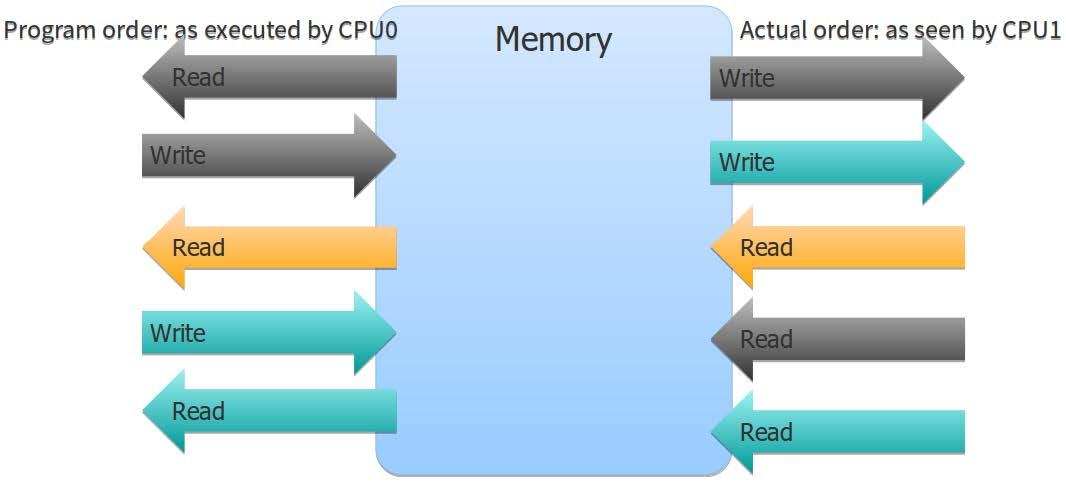
\includegraphics[width=0.9\textwidth]{content/1/chapter5/images/9.jpg}\\
Figure 5.9 – Visibility of operations with relaxed memory order
\end{center}

This is the visibility that we were talking about earlier: one CPU executes operations in a certain order, but their results are visible to other CPUs in a very different order. For brevity, we usually talk about the visibility of the operations and do not mention results every time.

If our operations on the shared counter N were executed with relaxed memory order, we would be in deep trouble: the only way to make our program correct would be to lock it so only one thread, the producer or the consumer, can run at any time, and we get no performance improvement from concurrency.

Fortunately, there are other memory order guarantees we can use. The most important one is the acquire-release memory order. When an atomic operation is executed with this order, we have a guarantee that any operation that accesses the memory and was executed before the atomic operation becomes visible to another thread before that thread executes an atomic operation on the same atomic variable. Similarly, all operations that are executed after the atomic operation become visible only after an atomic operation on the same variable. Again, remember that when we talk about the visibility of operations, we really mean that their results become observable to other CPUs. This is evident in Figure 5.10: on the left, we have the operations as they are executed by CPU0. On the right, we have the same operations as they are seen by CPU1. Note, in particular, that the atomic operation shown on the right is Atomic Write. But CPU1 does not execute atomic write: it executes an atomic read to see the results of the atomic write executed by CPU0. The same goes for all other operations: on the left, the order is as executed by CPU0. On the right, the order is as seen by CPU1.

%\hspace*{\fill} \\ %插入空行
\begin{center}
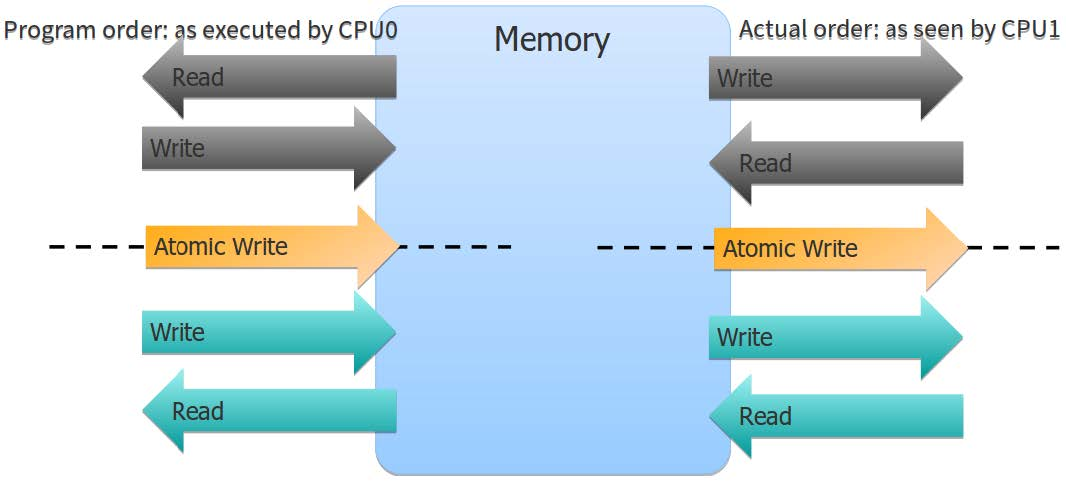
\includegraphics[width=0.9\textwidth]{content/1/chapter5/images/10.jpg}\\
Figure 5.10 – Visibility of operations with acquire-release memory order
\end{center}

The acquire-release order guarantee is a terse statement packed with a lot of important information, so let us elaborate on a few distinct points. First of all, the order is defined relative to the operations both threads execute on the same atomic variable. Until two threads access the same variable atomically, their clocks remain entirely arbitrary with respect to each other, and we cannot reason about what happens before or after something else, there is no meaning to these words. It is only when one thread has observed the results of an atomic operation executed by another thread that we can talk about before and after. In our producer-consumer example, the producer atomically increments the counter N. The consumer atomically reads the same counter. If the counter has not changed, we don't know anything about the state of the producer. But if the consumer sees that the counter has changed from N to N+1 and both threads use the acquire-release memory order, we know that all operations executed by the producer prior to incrementing the counter are now visible to the consumer. These operations include all the work necessary to construct the object that now resides in the array element buffer[N], and, thus, the consumer can safely access it.

The second salient point is that both threads must use the acquire-release memory order when accessing the atomic variable. If the producer uses this order to increment the count, but the consumer reads it with relaxed memory order, there are no guarantees on the visibility of any operations.

The final point is that all order guarantees are given in terms of before and after the operation on the atomic variable. Again, in our producer-consumer example, we know that the results of the operations executed by the producer to construct the Nth object are all visible by the consumer when it sees the counter change. There are no guarantees on the order in which these operations become visible. You can see this in Figure 5.10. Of course, it should not matter to us: we can't touch any part of the object until it's constructed, and, once the construction is finished, we don't care about the order in which it was done. The atomic operations with memory order guarantees act as barriers across which other operations cannot move. You can imagine such a barrier in Figure 5.10, dividing the entire program into two distinct parts: everything that happened before the count was incremented and everything that happened after. For that reason, it is often convenient to talk about such atomic operations as memory barriers.

Let us assume, for a moment, that in our program, all atomic operations on the counter N have acquire-release barriers. That would certainly guarantee that the program is correct. Note, however, that the acquire-release order is overkill for our needs. For the producer, it gives us the guarantee that all objects buffer[0] through buffer[N] that were constructed before we incremented the count to N+1 will be visible to the consumer when it sees the counter change from N to N+1. We need that guarantee. But we also have the guarantee that none of the operations executed for the purpose of constructing the remaining objects, buffer[N+1] and beyond, have become visible yet. We don't care about that: the consumer is not going to access these objects until it sees the next value of the counter. Similarly, on the consumer side, we have the guarantee that all the operations executed after the consumer sees the counter change to N+1 will have their effects (memory accesses) happen after that atomic operation. We need that guarantee: we do not want the CPU to reorder our consumer operations and execute some of the instructions that access the object buffer[N] before it is ready. But we also have the guarantee that the work done by the consumer to process the previous objects like buffer[N-1] is done and made visible to all threads before the consumer moves to the next object. Again, we don't need that guarantee: nothing depends on it.

What is the harm in having stronger guarantees than what is strictly necessary? In terms of correctness, none. But this is a book about writing fast programs (also, correct ones). Why are the ordering guarantees necessary in the first place? Because when left to their own devices, the compilers and the processors can reorder our program instructions almost arbitrarily. Why would they do that? Usually, to improve performance. Thus, it stands to reason that the more restrictions we impose on the ability to reorder the execution, the stronger the adverse impact on performance is. Therefore, in general, we want to use the memory order that is restrictive enough for the correctness of our program but no more strict than that.

The memory order that gives us exactly what we need for our producer-consumer program is as follows. On the producer side, we need one-half of the guarantee given by the acquire-release memory barrier: all operations executed before the atomic operation with the barrier must become visible to other threads before they execute the corresponding atomic operation. This is known as the release memory order:

%\hspace*{\fill} \\ %插入空行
\begin{center}
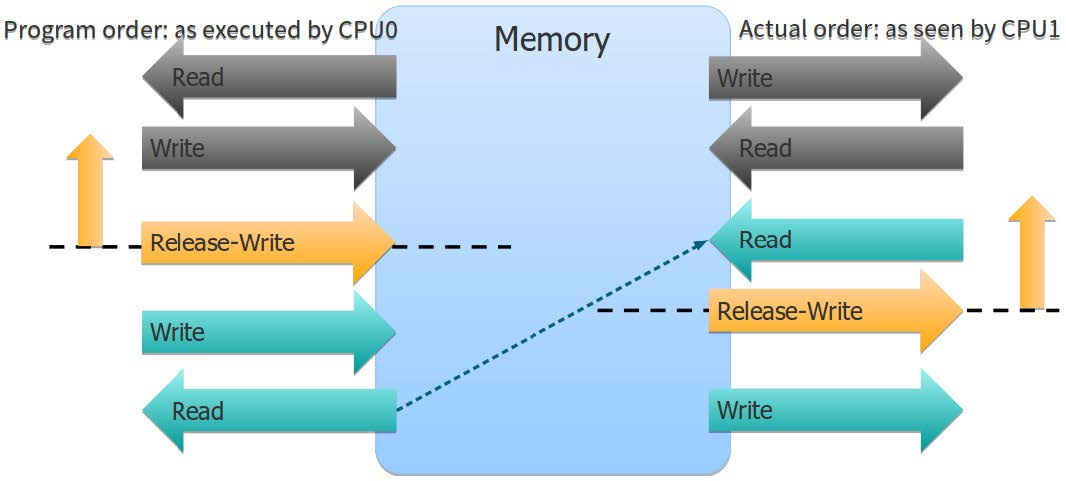
\includegraphics[width=0.9\textwidth]{content/1/chapter5/images/11.jpg}\\
Figure 5.11 – Release memory order
\end{center}

When CPU1 sees the result of the atomic write operation executed by CPU0 with the release memory order, it is guaranteed that the state of the memory, as seen by CPU1, already reflects all operations executed by CPU0 before this atomic operation. Note that we said nothing about the operations executed by CPU0 after the atomic operation. As we see in Figure 5.11, these operations may become visible in any order. The memory barrier created by the atomic operation is effective only in one direction: any operation that is executed before the barrier cannot cross it and be seen after the barrier. But the barrier is permeable in the other direction. For this reason, the release memory barrier and the corresponding acquire memory barrier are sometimes called half-barriers.

The acquire memory order is what we need to use on the consumer side. It guarantees that all operations executed after the barrier become visible to other threads after the barrier, as shown in Figure 5.12:

%\hspace*{\fill} \\ %插入空行
\begin{center}
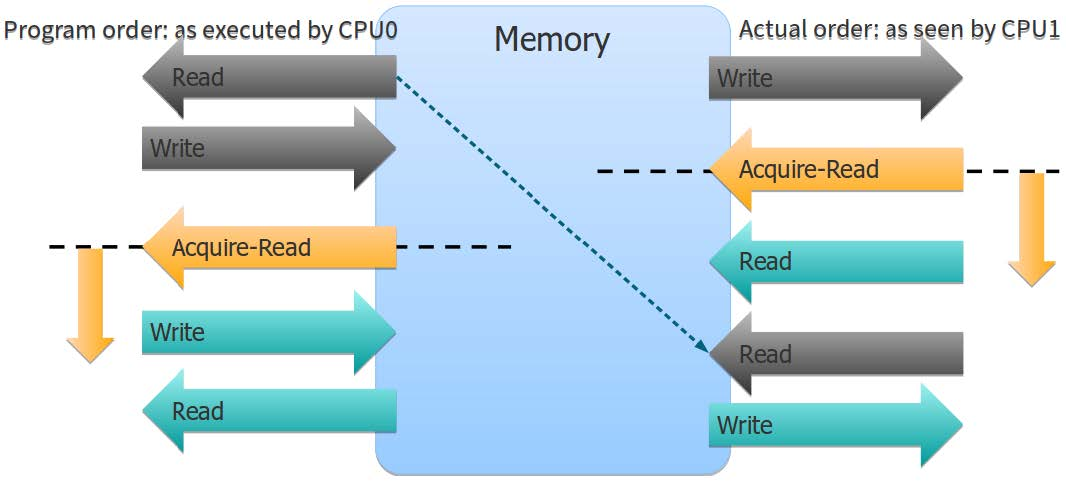
\includegraphics[width=0.9\textwidth]{content/1/chapter5/images/12.jpg}\\
Figure 5.12 – Acquire memory order
\end{center}

The acquire and release memory barriers are always used as a pair: if one thread (in our case, the producer) uses the release memory order with an atomic operation, the other thread (the consumer) must use the acquire memory order on the same atomic variable. Why do we need both barriers? On the one hand, we have the guarantee that everything that is done by the producer to build the new object before it increments the count is already visible to the consumer as soon as this increment is seen. But this is not enough, so, on the other hand, we have the guarantee that the operations executed by the consumer to process this new object cannot be moved backward in time, to a moment before the barrier when they could have seen the object in an unfinished state.

Now that we understand that it is not enough to just operate atomically on the shared data, you may ask whether our producer-consumer program actually works. As it turns out, both the lock version and the lock-free version are correct, even though we did not say anything explicitly about the memory order. So, how is the memory order controlled in C++?

\subsubsubsection{5.5.3\hspace{0.2cm}C++中的内存序}

First of all, let us think back to the lock-free version of our producer-consumer program, the one with the atomic counter:

\begin{lstlisting}[style=styleCXX]
std::atomic<size_t> N; // Count of initialized objects
T* buffer; // Only [0]…[N-1] are initialized
… Producer …
{
	new (buffer + N) T( … arguments … );
	++N; // Atomic, no need for locks
}
… Consumer …
for (size_t i = 0; keep_consuming(); ++i) {
	while (N <= i) {}; // Atomic read
	consume(buffer[i]);
}
\end{lstlisting}

The counter N is an atomic variable, an object of a type generated by the template std::atomic with the type parameter size\_t. All atomic types support atomic read and write operations, that is, they can appear in assignment operations. In addition, the integer atomics have the regular integer operations defined and implemented atomically, so ++N is an atomic increment (not all operations are defined, for example, there is no operator *=). None of these operations explicitly specify the memory order, so what guarantees do we have? As it turns out, by default, we get the strongest possible guarantee, the bidirectional memory barrier with each atomic operation (the actual guarantee is even a little stricter, as you will see in the next section). This is why our program is correct.

If you think this is overkill, you can reduce the guarantees to be just the ones you need, but you have to be explicit about it. The atomic operations can also be executed by calling the member functions of the std::atomic type, and that is where you can specify the memory order. The consumer thread needs a load operation with the acquire barrier:

\begin{lstlisting}[style=styleCXX]
while (N.load(std::memory_order_acquire) <= i);
\end{lstlisting}

The producer thread needs an increment operation with the release barrier (just like the increment operator, the member function also returns the value before the increment was done):

\begin{lstlisting}[style=styleCXX]
N.fetch_add(1, std::memory_order_release);
\end{lstlisting}

Before we go any further, we must realize that we have jumped over one critically important step in our optimization. The right way to start the previous paragraph is, If you think this is overkill, you have to prove it by performance measurements, and only then can you reduce the guarantees to be just the ones you need. Concurrent programs are hard enough to write even when using locks; the use of lock-free code and especially explicit memory orders has to be justified.

Speaking of locks, what memory order guarantees do they give? We know that any operation protected by the lock will be seen by any other thread that acquires the lock later, but what about the rest of the memory? The memory order enforced by the use of the lock is shown in Figure 5.13:

%\hspace*{\fill} \\ %插入空行
\begin{center}
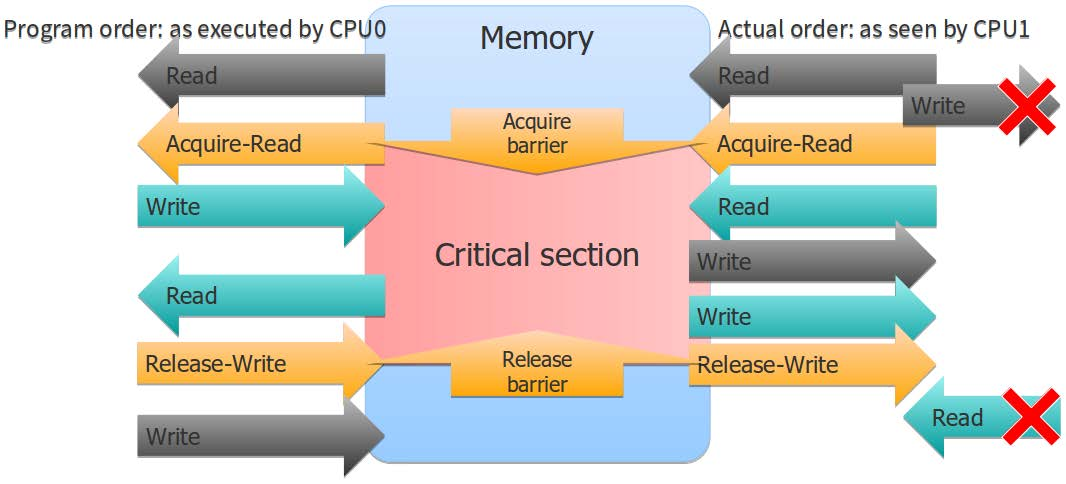
\includegraphics[width=0.9\textwidth]{content/1/chapter5/images/13.jpg}\\
Figure 5.13 – Memory order guarantees of a mutex
\end{center}

The mutexes have (at least) two atomic operations inside. Locking the mutex is an equivalent of a read operation with the acquire memory order (which explains the name: this is the memory order we use when we acquire the lock). The operation creates a half-barrier any operation executed earlier can be seen after the barrier, but any operation executed after the lock is acquired cannot be observed earlier. When we unlock the mutex or release the lock, the release memory order is guaranteed. Any operation executed before this barrier will become visible before the barrier. You can see that the pair of barriers, acquire and release, act as borders for the section of the code sandwiched between them. This is known as the critical section: any operation executed inside the critical section, that is, executed while the thread was holding the lock, will become visible to any other thread when it enters the critical section. No operation can leave the critical section (become visible earlier or later), but other operations from the outside can enter the critical section. Crucially, no such operation can cross the critical section: if an outside operation enters the critical section, it cannot leave. So, anything that was done by CPU0 before its critical section is guaranteed to be visible by CPU1 after its critical section.

For our producer-consumer program, this translates into the following guarantee:

\begin{lstlisting}[style=styleCXX]
… Producer …
new (buffer + N) T( … arguments … );
{ // Critical section start – acquire lock
	std::lock_guard l(mN);
	++N;
} // Critical section end - Release lock
… Consumer …
{ // Critical section – acquire lock
std::lock_guard l(mN);
n = N;
} // Critical section – release lock
consume(buffer[N]);
\end{lstlisting}

All operations executed by the producer to construct the Nth object are done before the producer enters the critical section. They will be visible to the consumer before it leaves its critical section and begins consuming the Nth object. Therefore, the program is correct.

The section you just read introduced the concept of memory order and illustrated it with examples. But, as you try to use this knowledge in your code, you will find the results wildly inconsistent. To better understand performance, what you should expect from the different ways you can use to synchronize your multi-threaded programs and avoid data races, we need to have a less hand-waving way to describe the memory order and related concepts.




































